\documentclass{report}

\usepackage[utf8]{inputenc} % Charakter-Kodierung
\usepackage[german]{babel} % Sprache

\usepackage[table,xcdraw]{xcolor} % Tabellen Farben
\usepackage{tabularx} % Dynamische Tabellenbreite
\usepackage{tcolorbox} % Graue Boxen
\usepackage{hyperref} % url Umgebung
\usepackage{todonotes} % Notizen
\usepackage{natbib} % Bibliographie
\usepackage{fancyhdr} % Header und Footer
\usepackage{multirow} % Multizeile
\usepackage{geometry} % Page layout
\usepackage{color} % Text Farben

\usepackage{enumitem}

% Page layout
\geometry{
	bottom=3.5cm,
	headheight=180pt
}

% Nummerierung der ersten Seiten verhindern
\pagenumbering{gobble}

% Bibstyle
\bibliographystyle{plain}

% Header / Footer
\fancypagestyle{plain}{
	\fancyhf{}% Clear header/footer
	\fancyhead[R]{\includegraphics[width=4cm]{img/cau-logo-2017}} % Rechter header
	\fancyhead[L]{\leftmark} % Linker header
	\fancyfoot[R]{\thepage} % Rechter footer
	\fancyfoot[L]{\includegraphics[width=1cm]{img/se-logo}} % Linker footer	
}
\pagestyle{plain}

\renewcommand{\headrulewidth}{0.5pt} % Unnötige Informationen der Kapitelangabe
\renewcommand{\footrulewidth}{0.2pt} % entfernen
\renewcommand{\chaptermark}[1]{\markboth{{#1}}{}}




% Zahlen für Fußnoten
\renewcommand{\thefootnote}{\arabic{footnote}}
\renewcommand{\thempfootnote}{\arabic{mpfootnote}}

%%%%% Ausfüllen %%%%%

% Gruppenname
\newcommand{\gruppenname}{Gruppe HRS 3 105b}

% Projektname
\newcommand{\projektname}{SWARM Composer}

% Semester
\newcommand{\semester}{SoSe18}



% Titelseite

\title{
	\vspace*{-3cm}
	Pflichtenheft\\
	\projektname\\
	-\\
	\color{gray}
	Softwareprojekt \semester\\
	\gruppenname\\
	\vspace*{5mm}
	
\includegraphics[width=\textwidth]{Logo/logo}
}

\author{
	\begin{tabular}{r l@{\hspace{8\tabcolsep}} r} 
		Jeremia & Böhmig & \multirow{8}{*}{ \includegraphics{img/se-logo} } \\
		Felix & Gröner \\
		Janek & Haberer \\
		Robert & Köhler \\
		Johanna & Menzel \\
		Jette & Petzold \\
		Christian & Richter \\
		Connor & Schönberner \\
	\end{tabular}
}

\date{\today}





% Dokument

\begin{document}
	\maketitle
	
	%%%% Bitte löschen oder auskommentieren %%%%
	%%%%%%%%% Dient nur als Hilfe %%%%%%%%%%
	
	
		
	%%%%%%%%%%%%%%%%%%%%%%%%%%%%%%
	
	\tableofcontents
	
	\chapter*{Einleitung}
	Dies ist das Pflichtenheft des SWARM Composers. Diese Software ist Teil des Forschungsprojektes SWARM des Unternehmens adesso.
	Der SWARM Composer dient dazu, unterschiedliche Software für Bauprojekte in Bezug auf ihre Kompatibilität bezüglich der Ein- und Ausgabeformate zu überprüfen.
	Der SWARM Composer besteht aus zwei Teilen: einem Webserver und einer App. Auf dem Webserver können BenutzerInnen Dienste zu Kompositionen zusammenfassen und auf Kompatibilität überprüfen. Neue Dienste können dabei manuell eingegeben oder durch eine JSON-Datei eingelesen werden. Dies ist aber nur mit Administratorrechten möglich. In der App können Kompositionen grafisch präsentiert und per Pdf verschickt werden.
	
	\noindent Unter einem \textbf{Dienst} wird ein Programm verstanden, das Daten in einem bestimmten Format einliest, diese verarbeitet und Daten in einem eventuell anderen Format ausgibt.
	
	\noindent Eine \textbf{Komposition} ist Zusammenfassung von Diensten mit der Information, welcher Dienst welchem anderen welche Daten sendet, und deren Kompatibilitätsbeziehungen.
	
	\noindent Zwei Dienste sind \textbf{kompatibel}, wenn das Eingabeformat des empfangenden Dienstes mit dem Ausgabeformat des sendenden Dienstes übereinstimmt.
	
	\noindent Wenn im Folgenden von \textbf{bearbeiten} die Rede ist, so beinhaltet dies stets auch das \textbf{Löschen}.
	
	
		
	
	\chapter{Lizenz}\label{chp:lizenz}
	\pagenumbering{arabic} % Nummerierung starten
	Copyright 2018 Jeremia B\"{o}hmig, Felix Gr\"{o}ner, Janek Haberer, Robert K\"{o}hler, Johanna Menzel, Jette Petzold, Christian Richter, Connor Sch\"{o}nberner \\
\\Lizenziert unter Apache License, der Version 2.0 (im Folgenden Lizenz); es ist nicht gestattet, die Software au\ss{}erhalb der durch die Lizenz festgelegten Bestimmungen zu verwenden.
Die volle Lizenz ist einsehbar unter
\begin{quote}
	http://www.apache.org/licenses/LICENSE-2.0 .
\end{quote}
Sofern nicht anders durch geltendes Gesetz vorgeschrieben oder schriftlich vereinbart, erfolgt die Verteilung der Software unter dieser Lizenz, so wie sie hier vorzufinden ist, ohne jedwede explizite oder implizite Garantien oder Bedingungen.
Zur Kenntnisnahme des genauen Wortlauts ist der volle Lizenztext unter dem angegebenen Link einzusehen.


	
	\chapter{Zielbestimmungen}\label{chp:zielbestimmungen}
	Im Folgenden ist der Funktionsumfang des SWARM Composers, insbesondere der Web-App und der Android-App, aufgeführt. Dabei werden funktionale und nicht-funktionale Zielbestimmungen getrennt aufgeführt. Des Weiteren wird zwischen Muss-, Soll-, Kann- und Abgrenzungskriterien unterschieden.
%
\begin{itemize}[leftmargin=4pc]
	\item Musskriterien umfassen alle Ziele und Funktionalitäten, die für einen Einsatz des entwickelten Produktes unabdingbar sind.
	Sie müssen daher ohne Kompromisse implementiert werden. Ein Wegfall eines einzelnen Musskriteriums würde das Produkt außer Betrieb setzen.
	\item Sollkriterien sind gewünschte Funktionen, die ebenfalls implementiert werden müssen, deren Wegfall auf Grund von unüblichen Umständen aber nicht den Einsatz des Produkts verhindern würde.
	\item Kannkriterien sind alle Ziele, die wünschenswert sind, aber nicht zwingend notwendige Funktionen darstellen. 
	\item Abgrenzungskriterien zeigen, was explizit \textbf{nicht} umgesetzt wird. Sie dienen dazu die Grenzen des Produkts zu definieren.
	\\\\
\end{itemize}
%

\textbf{Funktionale Zielbestimmungen}\newline
%

\textit{Musskriterium}

\begin{itemize}[leftmargin=4pc]
	\item Der SWARM Composer muss über eine native Android-App erreichbar sein.
	\item Der SWARM Composer muss über eine Website erreichbar sein.
	\item Es muss die Möglichkeit geben, über eine REST-Schnittstelle Dienste einzulesen.
	\item Beim manuellen Erstellen von Diensten, über eine Webmaske, muss das Format syntaktisch überprüft werden.
	\item Auf der Website muss die Möglichkeit bestehen, Kompositionen zu erstellen.
	\item Der SWAMP Composer muss eine Kompatibilitätsprüfung für Kompositionen durchführen.
	\item Es muss eine grafische Rückmeldung über die Kompatibilität von Diensten geben.
	\item Die Speicherung von erstellten Kompositionen muss möglich sein.
	\item Die Android-App muss erstellte Kompositionen anzeigen können.
	\item Neue Benutzer des SWARM Composers müssen über die Website registriert werden können.
	\item Registrierte Benutzer des SWARM Composers müssen sich anmelden können, unabhängig davon, ob sie über die Website oder die Android-App zugreifen.x
\end{itemize}

\textit{Sollkriterium}

\begin{itemize}[leftmargin=4pc]
	\item Unter allen Nutzern soll zwischen zwei Rollen, normaler Nutzer und Administrator, unterschieden werden, wobei letzterer mehr Nutzungsrechte hat.
	\item Die Website soll für Administratoren die Möglichkeit bieten, Dienste manuell dem System hinzuzufügen.
	\item Der Ersteller einer Komposition soll festlegen können, welche anderen Benutzer diese sehen können.
	\item Der Ersteller einer Komposition soll festlegen können, welche anderen Benutzer diese verändern können.
	\item In der Android-App soll die Möglichkeit bestehen, Kompositionen zu verschicken.
\end{itemize}

\textit{Kannkriterium}

\begin{itemize}[leftmargin=4pc]
	\item Die Android-App kann zu einzelnen Diensten die gespeicherten Informationen detailliert anzeigen.
	\item Es können Alternativen angezeigt werden, wenn Dienste nicht kompatibel sind.
	\item Es gibt eine Suchfunktion für Dienste und Kompositionen.
	\item Auf der Website können Kompositionen verschickt werden.
\end{itemize}

\textit{Abgrenzungskriterium}

\begin{itemize}[leftmargin=4pc]
	\item In der Android-App können keine Kompositionen erstellt werden.
	\item In der Android-App können keine Dienste erstellt werden.
	\item In der Android-App können keine Benutzer registriert werden.
	\item Beim manuellen Erstellen von Diensten wird nicht geprüft, ob der Inhalt korrekt ist.
	\item Es gibt keine benutzerspezifischen Einschränkungen bei der Sichtbarkeit einzelner Dienste. \\
\end{itemize}


\textbf{nicht funktionale Zielbestimmungen}\newline

\textit{Musskriterium}

\begin{itemize}[leftmargin=4pc]
	\item Die Web-Applikation muss mit Java-Spring erstellt werden.
	\item Die Android-App muss ab der Android Version 6 benutzbar sein.
	\item Die verwendeten URLs müssen zur Laufzeit änderbar sein.
\end{itemize}

\textit{Sollkriterium}

\begin{itemize}[leftmargin=4pc]
	\item Die Kommunikation zwischen Web-App und Android-App soll veschlüsselt sein.
	\item Es soll eine Drag and Drop Benutzeroberfläche auf der Website geben.
	\item Die Benutzeroberfläche soll einfach und intuitiv gestaltet sein.
	\item Der Quellcode des SWARM Composers soll unter eine geeignete Lizenz gestellt werden.
\end{itemize}


	
	\chapter{Produkteinsatz}\label{chp:produkteinsatz}
	\begin{tcolorbox}
In diesem Kapitel werden die folgenden drei Punkte erläutert:
\begin{enumerate}
	\item \textit{Anwendungsgebiete:} Was ist der Zweck des Produkts?
	\item \textit{Zielgruppen:} Für welche Benutzer (oder auch Rollen) ist das Produkt bestimmt?
	Welche Qualifikationen brauchen die Personen?
	\item \textit{Betriebsbedingungen:} Ist eine bestimmte physikalische Umgebung notwendig? 
	Wie ist die tägliche Betriebszeit des Produkts? 
	Automatische oder manuelle Datensicherung? 
	Autonomer oder beobachtender Betrieb?
\end{enumerate}

\noindent Der Teile des Produkteinsatzes werden üblicherweise als Fließtexte geschrieben.
\end{tcolorbox}
\section*{Anwendungsgebiete}
Der BIMSWARM Composer dient Anwender*Innen des BIMSWARM-Ökosystems dazu, Kombinationen von Diensten auf ihre Kompatibilität zu prüfen. Über das Ergebnis dieser Prüfung gibt das System grafisch eine Rückmeldung. Gleichzeitig lässt sich mit ihm ein Überblick über die vorhandenen atomaren Dienste erlangen sowie Kombinationen verwalten. 

\section*{Zielgruppen}

Primär richtet sich der BIMSWARM Composer an Benutzer*Innen aus der Architektur- und Baubranche, ohne dass weiteres Zusatzwissen über die interne Funktionsweise des Systems vorausgesetzt ist. Allerdings ist Wissen über übliche Services, die im BIMSWARM-Ökosystem genutzt werden, hiflreich, um Kombinationen zu erstellen.

Es sind zwei Rollen vorgesehen: Zum einen an Standard-User, die sowohl Dienste zu Kombinationen zusammensetzen als auch diese prüfen, speichern und teilen, zum anderen an Admin-User, die zusätzlich Dienste anlegen können. Ein Admin muss hierfür das von Adesso spezifizierte Format für Dienste kennen.

\section*{Betriebsumgebungen}

Zum Betrieb des Systems ist ein Server-Computer, auf dem die Webanwendung laufen kann, zwingend notwendig. Wenn die Nutzung der App gewünscht ist, ist hierfür ein Android-Mobilgerät in Form eines Tablets oder Smartphones notwendig. Für die auf einem Server (beispielsweise in Form von Apache Tomcat) laufende Anwendung ist ganztägige Uptime und autonomes Laufen gewährleistet. Es findet automatische Datensicherung statt.





		
	\chapter{Produktumgebung}\label{chp:produktumgebung}
	Um die Software fehlerfrei und korrekt zu nutzen, müssen bestimmte technische Bedingungen erfüllt sein, die hier aufgeführt werden.

\section{Software}

Für das Webinterface dient ein einfacher Webbrowser als Client.
Um die App zu benutzen, wird Android 6.0 oder neuer vorausgesetzt.
\newline
\newline
Auf dem Server muss eine Linux-Distribution mit Docker und Jenkins installiert sein.

\section{Hardware}

Für die App muss das Gerät Android 6.0 oder neuer unterstützen.
\newline
\newline
Webservices müssen auf dem Server laufen können.


\section{Orgware}

Sowohl Server als auch die Clients müssen netzwerkfähig sein.


\section{Produktschnittstelle}

Die Kommunikation zwischen Server und Client findet bei dem Webinterface über HTTPS und bei der App über eine REST-Schnittstelle statt. Für das Verschicken von wxxportierten Pdfs wird die Standard Android API verwendet.
	

	\chapter{Produktfunktionen}\label{chp:produktfunktionen}
	Die Produktfunktionen beschreiben jede einzelne Funktion des Produkts mittels Anwendungsfalldiagrammen und Anwendungsfalltabellen.
\\\\
In  Tabelle~\autoref{fig:akteur-tabelle} werden alle auftretenden Akteure beschrieben.


\begin{figure}[h]
	\centering

	\begin{tabularx}{\textwidth}{ p{.2\textwidth} | p{.4\textwidth} | X }
		\textbf{Akteur} & \textbf{Beschreibung} & \textbf{Verwendet in Anwendungsszenario} \\ \hline
		unregistrierteR NutzerIn & Nicht angemeldeter NutzerIn. Kann nur Kompositionen einsehen & APP-2, APP-3, WEB-6
		\\ \hline NutzerIn & Angemeldeter NutzerIn. Nutzt den SWARM Composer & APP-1, APP-2, APP-3, APP-4, WEB-4, WEB-5, WEB-6
		\\ \hline AdministratorIn & Nutzt und verwaltet den SWARM-Composer & APP-1, APP-2, APP-3, APP-4, WEB-1, WEB-2, WEB-3, WEB-4, WEB-5, WEB-6
	\end{tabularx}

	\caption{Beschreibung der Akteure}
	\label{fig:akteur-tabelle}
\end{figure}


%%%%%%%%%%%%%%%
%% Anwendungsfall 1 %%
%%%%%%%%%%%%%%%
\newpage

\section{Anwendungsfalldiagramm - App}

\begin{figure}[h]
	\centering	
	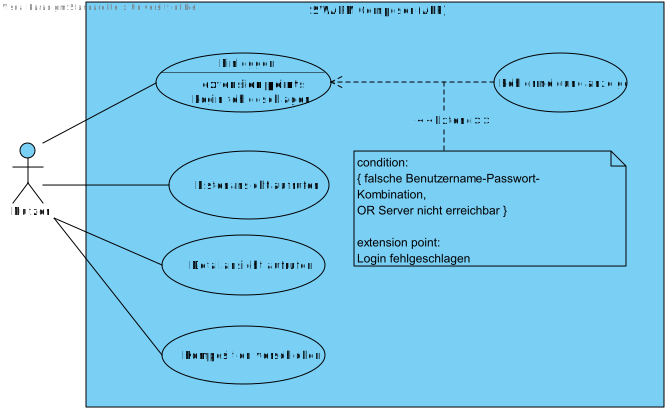
\includegraphics[width=\textwidth]{img/Produktfunktionen_app}	
	\caption{Anwendungsfalldiagramm - App}
	\label{fig:anwendungsfalldiagramm-app}
\end{figure}

\newpage

\begin{figure}[h]
	\centering
	\begin{tabularx}{\textwidth}{ X | X }
		\textbf{Anwendungsfall ID} & APP-1 \\ \hline
		\textbf{Anwendungsfallname} & Einloggen \\ \hline
		\textbf{Initiierender Akteur} & NutzerIn \\ \hline
		\textbf{Weitere Akteure} & -  \\ \hline
		\textbf{Kurzbeschreibung} & Der Nutzer loggt sich ein.  \\ \hline
		\textbf{Vorbedingungen} & Die Android-App ist geöffnet. Der Nutzer ist nicht eingeloggt.  \\ \hline
		\textbf{Nachbedingungen} & Der Nutzer ist eingeloggt.  \\ \hline
		\textbf{Ablauf} &
			\begin{enumerate}
				\item Der Nutzer gibt seinen Benutzernamen ein.
				\item Der Nutzer gibt sein Passwort ein.
				\item Der Nutzer tippt auf den Login-Button.
				\item Eine Bestätigung der erfolgreichen Anmeldung wird angezeigt.
			\end{enumerate} \\ \hline
		\textbf{Alternative} &
				- \\ \hline
		\textbf{Ausnahme} &
				\begin{enumerate}
					\item Der Nutzer gibt seinen Benutzernamen ein.
					\item Der Nutzer gibt sein Passwort ein.
					\item Der Nutzer tippt auf den Login-Button.
					\item Die Anmeldung schlägt fehl und eine Fehlermeldung wird angezeigt.
				\end{enumerate}  \\ \hline
		\textbf{Benutzte Anwendungsfälle} & Fehlermeldung anzeigen \\ \hline
		\textbf{Spezielle Anforderungen} & - \\ \hline
		\textbf{Annahmen} & -
	\end{tabularx}
	\caption{Anwendungsfall APP-1}
	\label{fig:anwendungsfall-app-tabelle-APP-1}
\end{figure}

\newpage

\begin{figure}[h]
	\centering
	\begin{tabularx}{\textwidth}{ X | X }
		\textbf{Anwendungsfall ID} & APP-2 \\ \hline
		\textbf{Anwendungsfallname} & Listenansicht aufrufen \\ \hline
		\textbf{Initiierender Akteur} & NutzerIn \\ \hline
		\textbf{Weitere Akteure} & -  \\ \hline
		\textbf{Kurzbeschreibung} & Dem Nutzer wird eine Liste von vorhandenen Kompositionen angezeigt.  \\ \hline
		\textbf{Vorbedingungen} & Die App ist geöffnet.  \\ \hline
		\textbf{Nachbedingungen} & Dem Nutzer wird eine Liste von vorhandenen Kompositionen angezeigt.  \\ \hline
		\textbf{Ablauf} &
		\begin{enumerate}
			\item Die für den Nutzer sichtbaren Kompositionen werden vom Server abgerufen.
			\item Die Daten werden als Liste angezeigt.
		\end{enumerate} \\ \hline
		\textbf{Alternative} &
		\begin{enumerate}
			\item Der Nutzer kehrt zur Listenansicht zurück.
			\item Ihm wird eine Liste der für ihn sichtbaren Kompositionen angezeigt.
		\end{enumerate}  \\ \hline
		\textbf{Ausnahme} &
		-  \\ \hline
		\textbf{Benutzte Anwendungsfälle} & - \\ \hline
		\textbf{Spezielle Anforderungen} & - \\ \hline
		\textbf{Annahmen} & -
	\end{tabularx}
	\caption{Anwendungsfall APP-2}
	\label{fig:anwendungsfall-app-tabelle-APP-2}
\end{figure}

\newpage

\begin{figure}[h]
	\centering
	\begin{tabularx}{\textwidth}{ X | X }
		\textbf{Anwendungsfall ID} & APP-3 \\ \hline
		\textbf{Anwendungsfallname} & Detailansicht aufrufen \\ \hline
		\textbf{Initiierender Akteur} & NutzerIn \\ \hline
		\textbf{Weitere Akteure} & -  \\ \hline
		\textbf{Kurzbeschreibung} & Der Nutzer ruft die Detailansicht einer Komposition auf.  \\ \hline
		\textbf{Vorbedingungen} & Der Nutzer hat die Listenansicht aufgerufen.  \\ \hline
		\textbf{Nachbedingungen} & Dem Nutzer wird die Detailansicht einer Komposition gezeigt.  \\ \hline
		\textbf{Ablauf} &
		\begin{enumerate}
			\item Der Nutzer wählt in der Listenansicht eine Komposition aus.
			\item Dem Nutzer werden die Details der ausgewählten Komposition angezeigt.
		\end{enumerate} \\ \hline
		\textbf{Alternative} &
		-  \\ \hline
		\textbf{Ausnahme} &
		- \\ \hline
		\textbf{Benutzte Anwendungsfälle} & - \\ \hline
		\textbf{Spezielle Anforderungen} & - \\ \hline
		\textbf{Annahmen} & -
	\end{tabularx}
	\caption{Anwendungsfall APP-3}
	\label{fig:anwendungsfall-app-tabelle-APP-3}
\end{figure}

\newpage

\begin{figure}[h]
	\centering
	\begin{tabularx}{\textwidth}{ X | X }
		\textbf{Anwendungsfall ID} & APP-4 \\ \hline
		\textbf{Anwendungsfallname} & Komposition verschicken \\ \hline
		\textbf{Initiierender Akteur} & Nutzer \\ \hline
		\textbf{Weitere Akteure} & -  \\ \hline
		\textbf{Kurzbeschreibung} & Der Nutzer verschickt eine Komposition.  \\ \hline
		\textbf{Vorbedingungen} & Der Nutzer hat in der Listenansicht eine Komposition ausgewählt und die Detailansicht aufgerufen.  \\ \hline
		\textbf{Nachbedingungen} & Die Komposition wird verschickt.  \\ \hline
		\textbf{Ablauf} &
		\begin{enumerate}
			\item Dem Nutzer wird eine Komposition in der Detailansicht angezeigt.
			\item Der Nutzer tippt auf den Verschicken-Button.
			\item Eine Datei im PDF-Format wird erstellt.
			\item Der Nutzer bestätigt den Versand.
		\end{enumerate} \\ \hline
		\textbf{Alternative} &
		-  \\ \hline
		\textbf{Ausnahme} &
		- \\ \hline
		\textbf{Benutzte Anwendungsfälle} & - \\ \hline
		\textbf{Spezielle Anforderungen} & - \\ \hline
		\textbf{Annahmen} & -
	\end{tabularx}
	\caption{Anwendungsfall APP-4}
	\label{fig:anwendungsfall-app-tabelle-APP-4}
\end{figure}

\newpage

%%%%%%%%%%%%%%%
%% Anwendungsfall 2 %%
%%%%%%%%%%%%%%%

\section{Anwendungsfalldiagramm - Server}

\begin{figure}[h]
	\centering
	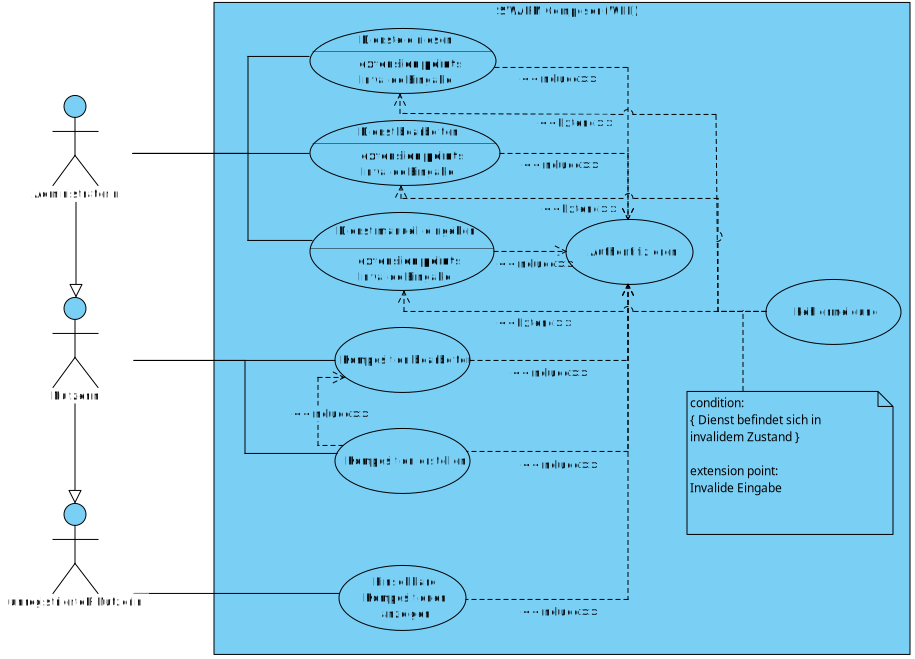
\includegraphics[width=\textwidth]{img/Produktfunktionen_web}
	\caption{Anwendungsfalldiagramm - Server}
	\label{fig:anwendungsfalldiagramm-server}
\end{figure}

\newpage

\begin{figure}[h]
	\centering
	\begin{tabularx}{\textwidth}{ X | X }
		\textbf{Anwendungsfall ID} & WEB-1 \\ \hline
		\textbf{Anwendungsfallname} & Dienst manuell einfügen \\ \hline
		\textbf{Initiierender Akteur} & AdministratorIn \\ \hline
		\textbf{Weitere Akteure} & - \\ \hline
		\textbf{Kurzbeschreibung} & Ein neuer Dienst wird in die Datenbank eingefügt. \\ \hline
		\textbf{Vorbedingungen} & AdministratorIn ist eingeloggt und befindet sich auf Administrationsseite. \\ \hline
		\textbf{Nachbedingungen} & Neuer Dienst wurde in Datenbank gespeichert. \\ \hline
		\textbf{Ablauf} &
		\begin{enumerate}
			\item [1.] [Use-Case: Authentifizieren]
			\item [2.] AdministratorIn wählt ``Dienst eingeben'' aus.
			\item [3.] AdministratorIn gibt Dienstdetails in Eingabemaske ein.
			\item [4.] AdministratorIn bestätigt die Eingabe.
			\item [5.] System akzeptiert Eingabe und speichert in Datenbank.
			\item [6.] Zurück zur Administrationsseite.
		\end{enumerate} \\ \hline
		\textbf{Alternative} & - \\ \hline
		\textbf{Ausnahme} &
		\begin{enumerate}
			\item [1.] [Use-Case: Authentifizieren]
			\item [2.] AdministratorIn wählt ``Dienst eingeben'' aus.
			\item [3.] AdministratorIn gibt Dienstdetails in Eingabemaske ein.
			\item [4.] AdministratorIn bestätigt seine Eingabe.
			\item [5.] System akzeptiert Eingabe nicht, da sie invalide ist.
			\item [6.] System zeigt Fehler an und markiert invalide Felder.
			\item [7.] Es wird in der Eingabemaske verblieben.
		\end{enumerate} \\ \hline
		\textbf{Benutzte Anwendungsfälle} & Authentifizieren \\ \hline
		\textbf{Spezielle Anforderungen} & - \\ \hline
		\textbf{Annahmen} & Die Authentifizierung ist erfolgreich.
	\end{tabularx}
	\caption{Anwendungsfall WEB-1}
	\label{fig:anwendungsfall-server-tabelle-web-1}
\end{figure}

\begin{figure}[h]
	\centering
	\begin{tabularx}{\textwidth}{ X | X }
		\textbf{Anwendungsfall ID} & WEB-2 \\ \hline
		\textbf{Anwendungsfallname} & Dienste einlesen \\ \hline
		\textbf{Initiierender Akteur} & AdministratorIn \\ \hline
		\textbf{Weitere Akteure} & - \\ \hline
		\textbf{Kurzbeschreibung} & Ein oder mehrere Dienste werden über eine JSON Datei eingelesen, die sich lokal auf einem Nutzerrechner befindet. \\ \hline
		\textbf{Vorbedingungen} & AdministratorIn ist eingeloggt und befindet sich auf Administrationsseite. \\ \hline
		\textbf{Nachbedingungen} & Neue Dienste wurden der Datenbank hinzugefügt. \\ \hline
		\textbf{Ablauf} &
		\begin{enumerate}
			\item [1.] [Use-Case: Authentifizieren]
			\item [2.] AdministratorIn wählt ``Dienste einlesen'' aus.
			\item [3.] AdministratorIn wählt die hochzuladene JSON Datei aus dem sich öffnendem Dateibrowser vom lokalen Rechner aus.
			\item [4.] Eingelesene Daten werden vom System akzeptiert und aufgelistet.
			\item [5.] AdministratorIn speichert.
			\item [6.] Dienste werden in Datenbank gespeichert.
			\item [7.] Es erscheint die Administrationsseite.
		\end{enumerate} \\ \hline
		\textbf{Alternative} & - \\ \hline
		\textbf{Ausnahme} &
		\begin{enumerate}
			\item [1.]  [Use-Case: Authentifizieren]
			\item [2.]  AdministratorIn wählt ``Dienste einlesen'' aus.
			\item [3.]  AdministratorIn wählt hochzuladene JSON Datei aus dem sich öffnenden Dateibrowser vom lokalen Rechner aus.
			\item [4.]  System erkennt Fehler in der JSON Datei und gibt einen Fehler aus.
			\item [5.]  Administrator bleibt auf der Administrationseite.
		\end{enumerate}  \\ \hline
		\textbf{Benutzte Anwendungsfälle} & Authentifizieren \\ \hline
		\textbf{Spezielle Anforderungen} & - \\ \hline
		\textbf{Annahmen} & Die Authentifizierung ist erfolgreich.
	\end{tabularx}
	\caption{Anwendungsfall WEB-2}
	\label{fig:anwendungsfall-server-tabelle-web-2}
\end{figure}

\begin{figure}[h]
	\centering
	\begin{tabularx}{\textwidth}{ X | X }
		\textbf{Anwendungsfall ID} & WEB-3 \\ \hline
		\textbf{Anwendungsfallname} & Dienst bearbeiten \\ \hline
		\textbf{Initiierender Akteur} & AdministratorIn \\ \hline
		\textbf{Weitere Akteure} & - \\ \hline
		\textbf{Kurzbeschreibung} & Felder eines existierenden Dienstes werden bearbeitet. \\ \hline
		\textbf{Vorbedingungen} & AdministratorIn ist eingeloggt und befindet sich auf Administrationsseite. \\ \hline
		\textbf{Nachbedingungen} & Vorgenommene Änderungen am Dienst wurden in Datenbank übernommen. \\ \hline
		\textbf{Ablauf} &
		\begin{enumerate}
			\item [1.] [Use-Case: Authentifizieren]
			\item [2.] AdministratorIn wählt Dienst aus Liste von vorhandenen Diensten aus.
			\item [3.] AdministratorIn wählt ``Bearbeiten''.
			\item [4.] AdministratorIn führt Änderungen in Eingabemaske durch.
			\item [5.] AdministratorIn bestätigt die Eingabe.
			\item [6.] System akzeptiert die Änderung und speichert diese in der Datenbank.
		\end{enumerate} \\ \hline
		\textbf{Alternative} & - \\ \hline
		\textbf{Ausnahme} &
		\begin{enumerate}
			\item [1.] [Use-Case: Authentifizieren]
			\item [2.] AdministratorIn wählt Dienst aus Liste von vorhandenen Diensten aus.
			\item [3.] AdministratorIn wählt ``Bearbeiten''.
			\item [4.] AdministratorIn tätigt eine invalide Eingabe.
			\item [5.] AdministratorIn bestätigt die Eingabe.
			\item [6.] System erkennt Fehler und zeigt eine Fehlermeldung an.
			\item [6.] AdministratorIn bleibt auf der Administrationsseite.
		\end{enumerate}  \\ \hline
		\textbf{Benutzte Anwendungsfälle} & Authentifizieren \\ \hline
		\textbf{Spezielle Anforderungen} & - \\ \hline
		\textbf{Annahmen} & Die Authentifizierung ist erfolgreich.
	\end{tabularx}
	\caption{Anwendungsfall WEB-3}
	\label{fig:anwendungsfall-server-tabelle-web-3}
\end{figure}

\begin{figure}[h]
	\centering
	\begin{tabularx}{\textwidth}{ X | X }
		\textbf{Anwendungsfall ID} & WEB-4 \\ \hline
		\textbf{Anwendungsfallname} & Komposition erstellen \\ \hline
		\textbf{Initiierender Akteur} & NutzerIn \\ \hline
		\textbf{Weitere Akteure} & - \\ \hline
		\textbf{Kurzbeschreibung} & Eine neue Komposition wird zum System hinzugefügt. \\ \hline
		\textbf{Vorbedingungen} & NutzerIn befindet sich auf der Übersichtsseite und ist eingeloggt.  \\ \hline
		\textbf{Nachbedingungen} & Komposition ist erstellt und NutzerIn befindet sich im Bearbeitungsmodus. \\ \hline
		\textbf{Ablauf} &
		\begin{enumerate}
			\item[1.]  [Use-Case: Authentifizieren]
			\item[2.]  NutzerIn wählt ``Komposition erstellen'' aus.
			\item[3.]  NutzerIn gibt einen Namen für die Komposition an.
			\item[4.]  NutzerIn wird weitergeleitet zum Bearbeitungsmodus.
			\item[5.] [Use-Case: Komposition bearbeiten]
		\end{enumerate} \\ \hline
		\textbf{Alternative} & - \\ \hline
		\textbf{Ausnahme} & - \\ \hline
		\textbf{Benutzte Anwendungsfälle} & WEB-5, Authentifizieren\\ \hline
		\textbf{Spezielle Anforderungen} & - \\ \hline
		\textbf{Annahmen} & Die Authentifizierung ist erfolgreich.
	\end{tabularx}
	\caption{Anwendungsfall WEB-5}
	\label{fig:anwendungsfall-server-tabelle-web-4}
\end{figure}

\begin{figure}[h]
	\centering
	\begin{tabularx}{\textwidth}{ X | X }
		\textbf{Anwendungsfall ID} & WEB-5 \\ \hline
		\textbf{Anwendungsfallname} & Komposition bearbeiten \\ \hline
		\textbf{Initiierender Akteur} & NutzerIn \\ \hline
		\textbf{Weitere Akteure} & - \\ \hline
		\textbf{Kurzbeschreibung} & NutzerIn bearbeitet Komposition. \\ \hline
		\textbf{Vorbedingungen} & NutzerIn besitzt benötigte Rechte zur Bearbeitung der Komposition und befindet sich auf der Übersichtsseite. \\ \hline
		\textbf{Nachbedingungen} & NutzerIn befindet sich im Bearbeitungsmodus. \\ \hline
		\textbf{Ablauf} &
		\begin{enumerate}
			\item[1.] [Use-Case: Authentifizieren]
			\item[2.] NutzerIn wählt ``Komposition bearbeiten'' aus.
			\item[3.] NutzerIn wird in den Bearbeitungsmodus versetzt.
		\end{enumerate} \\ \hline
		\textbf{Alternative} & - \\ \hline
		\textbf{Ausnahme} & - \\ \hline
		\textbf{Benutzte Anwendungsfälle} & Authentifizieren \\ \hline
		\textbf{Spezielle Anforderungen} & - \\ \hline
		\textbf{Annahmen} & Es werden nur Komposition gezeigt für die der NutzerIn die benötigten Rechte besitzt.
                  Der Bearbeitungsbutton ist ausgegraut, falls die Bearbeitungsrechte nicht vorhanden sind. Die Authentifizierung war erfolgreich.
	\end{tabularx}
	\caption{Anwendungsfall WEB-5}
	\label{fig:anwendungsfall-server-tabelle-web-5}
\end{figure}

\begin{figure}[h]
	\centering
	\begin{tabularx}{\textwidth}{ X | X }
		\textbf{Anwendungsfall ID} & WEB-6 \\ \hline
		\textbf{Anwendungsfallname} & Einsehbare Komposition anzeigen \\ \hline
		\textbf{Initiierender Akteur} & unregistrierteR NutzerIn oder NutzerIn\\ \hline
		\textbf{Weitere Akteure} & - \\ \hline
		\textbf{Kurzbeschreibung} & (UnregistrierteR) NutzerIn  lässt sich eine Komposition anzeigen. \\ \hline
		\textbf{Vorbedingungen} & (UnregistrierteR) NutzerIn befindet sich auf der Übersichtsseite. \\ \hline
		\textbf{Nachbedingungen} & (UregistrierteR) NutzerIn wird die Komposition angezeigt. \\ \hline
		\textbf{Ablauf} &
		\begin{enumerate}
			\item[1.] [Use-Case: Authentifizieren]
			\item[2.] (UnregistrierteR) NutzerIn wählt die anzuzeigende Komposition aus.
			\item[3.] (UnregistrierteR) NutzerIn wird die Komposition angezeigt.
		\end{enumerate} \\ \hline
		\textbf{Alternative} & - \\ \hline
		\textbf{Ausnahme} & - \\ \hline
		\textbf{Benutzte Anwendungsfälle} & Authentifizieren \\ \hline
		\textbf{Spezielle Anforderungen} & - \\ \hline
		\textbf{Annahmen} & Es werden nur Kompositionen gezeigt, für die der (unregistrierteR) NutzerIn die benötigten Rechte besitzt. Die Authentifizierung war erfolgreich.
	\end{tabularx}
	\caption{Anwendungsfall WEB-6}
	\label{fig:anwendungsfall-server-tabelle-web-6}
\end{figure}

	\chapter{Testfälle}\label{chp:testfaelle}
	\begin{tcolorbox}
In diesem Abschnitt werden Testfälle für die Anwendungsfälle der Produktfunktionen definiert.
Diese sollen später ebenfalls als \textbf{reale Tests} implementiert werden.

\autoref{fig:testfaelle-tabelle} stellt eine exemplarische Tabelle für die Beschreibung der zu testenden Anwendungsfälle dar. 
Stil und Formatierung sind variabel.
\end{tcolorbox}

\begin{figure}[!h]
	\begin{center}
		\begin{tabularx}{\textwidth}{ p{.05\textwidth} | p{.25\textwidth} | p{.2\textwidth} | X }
			\textbf{Nr.} & \textbf{Anwendungsfall ID} & \textbf{Szenario} & \textbf{Erwartetes Verhalten} \\ \hline
			1 & XX-1 & Der Informatiker programmiert ... & Der Quellcode ist schön.\\ \hline
			2 & XX-2 & Der Informatiker trinkt Kaffee ... & Die Arbeitsleistung steigt.
		\end{tabularx}	
	\end{center}
	\caption{Beschreibung der Akteure}
	\label{fig:testfaelle-tabelle}
\end{figure}
	
	\chapter{Produktdaten}\label{chp:produktdaten}
	Zu den Benutzern werden folgende Daten gespeichert:
\begin{itemize}
	\item Name
	\item ID
	\item Passwort
	\item Erstellte Kompositionen
	\item Kompositionen, für die er Leserechte besitzt
	\item Kompositionen, für die er Schreibrechte besitzt
	\item Benutzergruppen, zu welchen er gehört.
\end{itemize}
Zu den Diensten werden folgende Daten gespeichert:
\begin{itemize}
	\item Name
	\item Organisation
	\item Version
	\item ID
	\item Schlagworte
	\item gültige Eingabeformate
	\item gültige Ausgabeformate
\end{itemize}
Zu den Kompositionen werden folgende Daten gespeichert:
\begin{itemize}
	\item Autor
	\item Enthaltene Dienste
	\item Benutzergruppen mit Leserechten
	\item Benutzergruppen mit Schreibrechten
\end{itemize}

Zu den Ein- und Ausgabeformaten werden folgende Daten:
\begin{itemize}
	\item Typ des Eingabeformats (z.B JSON)
	\item Version
	\item Abwärtskompatibilität
\end{itemize}
\\Bei der Abwärtskompatibilität wird zwischen \textit{strict} und \textit{flexible} unterschieden. Mit \textit{flexible} markierte Formate sind abwärtskompatibel, mit \textit{strict} gekennzeichnete hingegen nicht.

	
	\chapter{Benutzeroberfläche}\label{chp:benutzeroberflaeche}
	\begin{tcolorbox}
In diesem Kapitel werden erste Skizzen (Mockups) der Benutzeroberflächen dargestellt.
Diese sollen in erster Linie dazu dienen, dem Kunden einen Überblick über die zu erstellenden UIs zu geben und ggf. Änderungen frühzeitig durchführen zu können.
Dafür eignen sich spezielle Tools, wie z.B. Balsamiq Mockups\footnote{\url{https://balsamiq.com/products/mockups}}.
\end{tcolorbox}

\begin{figure}[h]
	\centering
	\missingfigure{Startbildschirm}		
	\caption{Startbildschirm}
	\label{fig:mock-start}
\end{figure}

\begin{figure}[h]
	\centering
	\missingfigure{Passwort ändern}		
	\caption{Passwort ändern}
	\label{fig:mock-pw}
\end{figure}
	
	\chapter{Qualitätsanforderung}\label{chp:qualitaetsanforderung}
	Die Tabelle \ref{tabelle:qualitaetsanforderungen} zeigt an, welche Eigentschaften der Software bei der Entwicklung mit welcher Priorität betrachtet wird.

\begin{table}[h]
	\centering
	\begin{tabularx}{\textwidth}{l c c c c}
		\rowcolor[HTML]{C0C0C0} 
		& \textbf{sehr wichtig} & \textbf{wichtig} & \textbf{weniger wichtig} & \textbf{unwichtig} \\
		Robustheit &  &  & x &  \\
		\rowcolor[HTML]{E7E7E7} 
		Zuverlässigkeit & x &  &  &  \\
		Wartbarkeit &  & x &  &  \\
		\rowcolor[HTML]{E7E7E7} 
		Erweiterbarkeit &  & x &  &  \\
		Benutzerfreundlichkeit & x &  &  &  \\
		\rowcolor[HTML]{E7E7E7} 
		Effizienz &  &  & x &  \\
		Anpassbarkeit &  &  & x &  \\
		\rowcolor[HTML]{E7E7E7} 
		Kompatibilität &  &  & x &  \\
		Sicherheit &  & x &  & 
	\end{tabularx}
	\caption{Qualitätsanforderungen}
	\label{tabelle:qualitaetsanforderungen}
\end{table}
	
	\chapter{Glossar}\label{chp:glossar}
	\begin{tcolorbox}
In diesem Glossar können Akronyme und abkürzende Schreibweisen aufgelistet werden. 
Alle verwendeten Abkürzungen innerhalb des Projekts müssen hier erläutert werden.
\end{tcolorbox}

\begin{table}[h]
	\centering
	\begin{tabularx}{\textwidth}{X X}
		\rowcolor[HTML]{C0C0C0} 
		\textbf{Abkürzung} & \textbf{Beschreibung} \\
		Abk. A & Beschreibung A \\
		\rowcolor[HTML]{E7E7E7} 
		Abk. B & Beschreibung B \\
		Abk. C & Beschreibung C \\
		\rowcolor[HTML]{E7E7E7} 
		Abk. D & Beschreibung D \\
		Abk. E & Beschreibung E \\
		\rowcolor[HTML]{E7E7E7} 
		Abk. F & Beschreibung F \\
		Abk. G & Beschreibung G
	\end{tabularx}
	\caption{Glossar}
	\label{table:glossar}
\end{table}
	
	\bibliography{references}
	\pagenumbering{gobble} % Nummerierung deaktivieren
	
\end{document}